\documentclass[14pt, a4paper]{extarticle}
\usepackage{style}
\usepackage{array}
\usepackage{biblatex}
\usepackage{amsmath}
\usepackage{indentfirst}
\usepackage{listings}
\usepackage{xcolor}
\usepackage{fefutitle}
\usepackage{listingFreeFem}

\lstset{
	columns=fullflexible,
	frame=single,
	numbers=left,
	numberstyle=\color{gray},
	breaklines=true,
	tabsize=2
}

\newcolumntype{P}[1]{>{\centering\arraybackslash}p{#1}}

\begin{document}
	
	\fefutitle{2}{Численная реализация вариационного метода штрафа в задаче интерполяции на произвольной сетке данных}
	\pagebreak
	
	\section{Введение}
	\section{Постановка задачи}
	\section{Алгоритм}
	\section{Вариационная постановка задачи}
		Для решения дифференциального уравнения с частными производными будем использовать метод конечных элементов, поэтому необходима вариационная постановка задачи.
		
		Умножим уравнение на тестовую функция \(v(x, y), v\rvert_\Gamma = g, u\in C^1(\Omega)\) с последующим интегрирование по области $\Omega$:
		\[ \int\displaylimits_{\Omega}-\Delta uvdxdy + 
		\dfrac{1}{\varepsilon^2}\sum_{i=1}^{n}\int\displaylimits_{\Omega}\delta_x\delta_yuvdxdy -
		\dfrac{1}{\varepsilon^2}\sum_{i=1}^{n}\int\displaylimits_{\Omega}\delta_x\delta_yfvdxdy = 0 \]
		
		Применим первую формулу Грина:
		\[ \int\displaylimits_{\Omega}\nabla u\nabla v dxdy - \int\displaylimits_{\Gamma}v\dfrac{du}{dn}d\Gamma +
		\dfrac{1}{\varepsilon^2}\sum_{i=1}^{n}\int\displaylimits_{\Omega}\delta_x\delta_yuvdxdy -
		\dfrac{1}{\varepsilon^2}\sum_{i=1}^{n}\int\displaylimits_{\Omega}\delta_x\delta_yfvdxdy = 0 \]
		
		Так как на границе задано условие Дирихле, то \( \int\displaylimits_{\Gamma}v\dfrac{du}{dn}d\Gamma = 0 \), получим:
		\[ \int\displaylimits_{\Omega}\nabla u\nabla v dxdy +
		\dfrac{1}{\varepsilon^2}\sum_{i=1}^{n}\int\displaylimits_{\Omega}\delta_x\delta_yuvdxdy -
		\dfrac{1}{\varepsilon^2}\sum_{i=1}^{n}\int\displaylimits_{\Omega}\delta_x\delta_yfvdxdy = 0 \]
	\section{Расчетная часть}
		\begin{enumerate}
			\item \( f(x, y) = 3\sin{x} + (y - 0.2)^2 \)
			
			\(N = 5774\)
			\begin{table}[H]
				\centering
				\begin{tabular}{|P{5cm}|P{2.5cm}|P{2.5cm}|P{2.5cm}|}
					\hline
					M & 10 & 25 & 50 \\ \hline
					Относительная погрешность & $0.008963$ & $0.008207$ & $0.007454$\\ \hline
				\end{tabular}
			\end{table}
			
			\(M = 25\)
			\begin{table}[H]
				\centering
				\begin{tabular}{|P{5cm}|P{2.5cm}|P{2.5cm}|P{2.5cm}|}
					\hline
					N & 3718 & 5774 & 17101 \\ \hline
					Относительная погрешность & 0.032763 & 0.008207 & 0.0067239\\ \hline
				\end{tabular}
			\end{table}
		
			\begin{figure}[H]
				\begin{minipage}{0.5\textwidth}
					\centering
					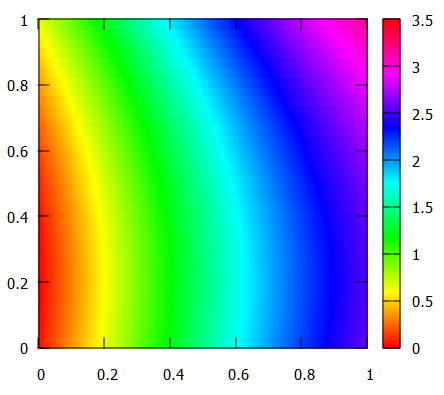
\includegraphics[width = \linewidth]{../1func/imOrig1.png}
					\caption[.] {Интерполируемая функция}
				\end{minipage}\hfill
				\begin{minipage}{0.5\textwidth}
					\centering
					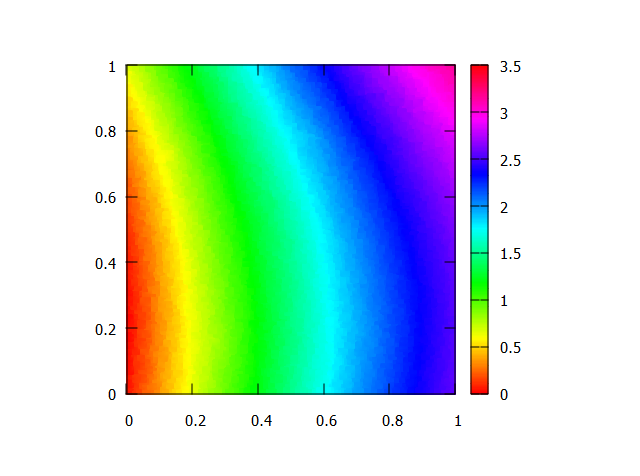
\includegraphics[width = \linewidth]{../1func/M=10T=5774Err=0.008963.png}
					\caption[.] {Интерполяци при 10 точках}
				\end{minipage}\hfill
			\end{figure}
			\begin{figure}[H]
				\begin{minipage}{0.5\textwidth}
					\centering
					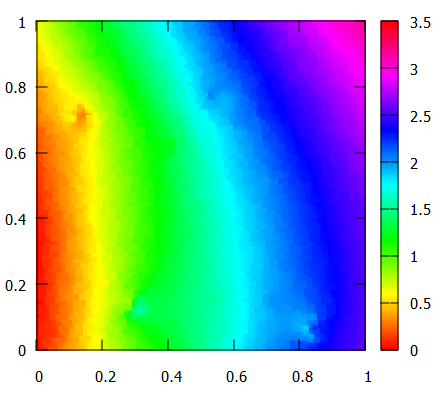
\includegraphics[width = \linewidth]{../1func/M=25T=3718Err=0.032763.png}
					\caption[.] {Интерполяция при 25 точках с редкой сеткой}
				\end{minipage}\hfill
				\begin{minipage}{0.5\textwidth}
					\centering
					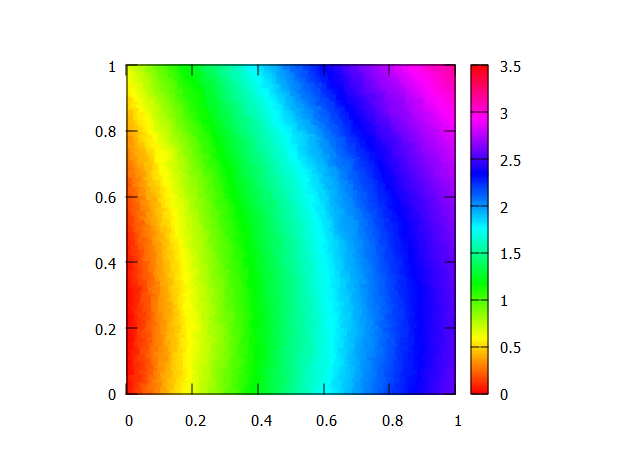
\includegraphics[width = \linewidth]{../1func/M=25T=5774Err=0.008207.png}
					\caption[.] {Интерполяция при 25 точках}
				\end{minipage}\hfill
			\end{figure}
			\begin{figure}[H]
				\begin{minipage}{0.5\textwidth}
					\centering
					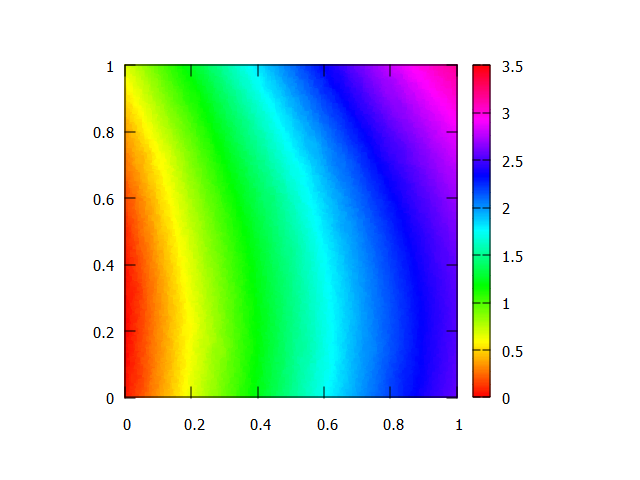
\includegraphics[width = \linewidth]{../1func/M=25T=17101Err=0.0067239.png}
					\caption[.] {Интерполяция при 25 точках с частой сеткой}
				\end{minipage}\hfill
				\begin{minipage}{0.5\textwidth}
					\centering
					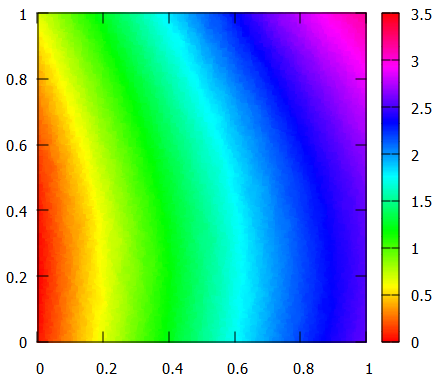
\includegraphics[width = \linewidth]{../1func/M=50T=5774Err=0.007454.png}
					\caption[.] {Интерполяция при 50 точках}
				\end{minipage}\hfill
			\end{figure}
		
			\item \( f(x, y) = \arctan{(10(x + y))} \)
			
			\(N = 5774\)
			\begin{table}[H]
				\centering
				\begin{tabular}{|P{5cm}|P{2.5cm}|P{2.5cm}|P{2.5cm}|}
					\hline
					M & 10 & 25 & 50 \\ \hline
					Относительная погрешность & $0.0223348$ & $0.0170492$ & $0.013383$\\ \hline
				\end{tabular}
			\end{table}
			
			\(M = 25\)
			\begin{table}[H]
				\centering
				\begin{tabular}{|P{5cm}|P{2.5cm}|P{2.5cm}|P{2.5cm}|}
					\hline
					N & 3718 & 5774 & 17101 \\ \hline
					Относительная погрешность & 0.0168654 & 0.0170492 & 0.0163659\\ \hline
				\end{tabular}
			\end{table}
			
			\begin{figure}[H]
				\begin{minipage}{0.5\textwidth}
					\centering
					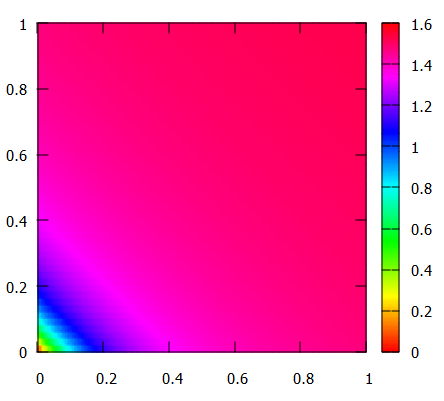
\includegraphics[width = \linewidth]{../2func/orig.png}
					\caption[.] {Интерполируемая функция}
				\end{minipage}\hfill
				\begin{minipage}{0.5\textwidth}
					\centering
					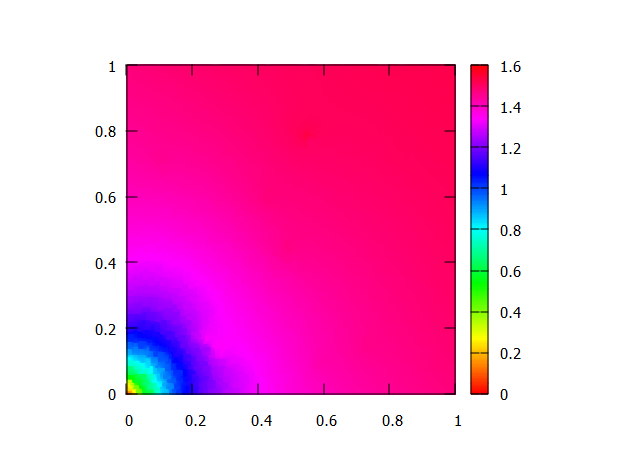
\includegraphics[width = \linewidth]{../2func/M=10T=5774Err=0.022348.png}
					\caption[.] {Интерполяци при 10 точках}
				\end{minipage}\hfill
			\end{figure}
			\begin{figure}[H]
				\begin{minipage}{0.5\textwidth}
					\centering
					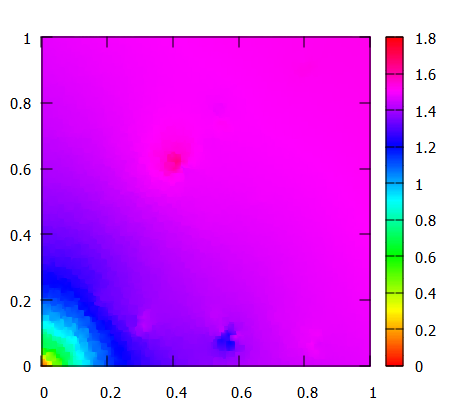
\includegraphics[width = \linewidth]{../2func/M=25T=3718Err=0.0168654.png}
					\caption[.] {Интерполяция при 25 точках с редкой сеткой}
				\end{minipage}\hfill
				\begin{minipage}{0.5\textwidth}
					\centering
					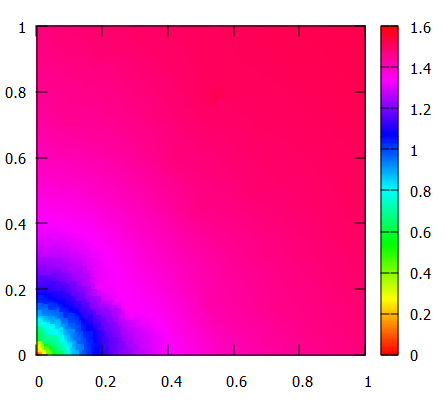
\includegraphics[width = \linewidth]{../2func/M=25T=5774Err=0.0170492.png}
					\caption[.] {Интерполяция при 25 точках}
				\end{minipage}\hfill
			\end{figure}
			\begin{figure}[H]
				\begin{minipage}{0.5\textwidth}
					\centering
					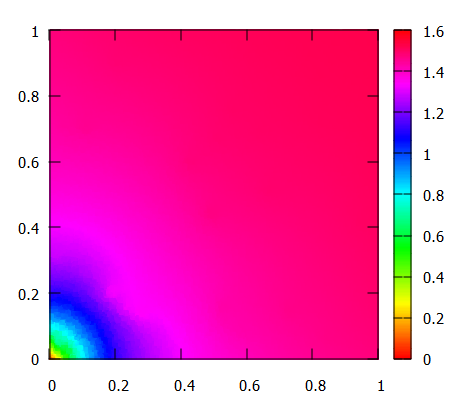
\includegraphics[width = \linewidth]{../2func/M=25T=17101Err=0.0163659.png}
					\caption[.] {Интерполяция при 25 точках с частой сеткой}
				\end{minipage}\hfill
				\begin{minipage}{0.5\textwidth}
					\centering
					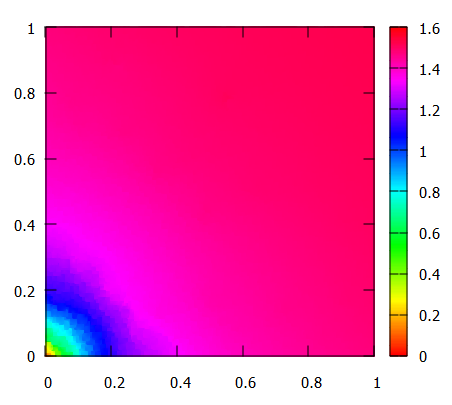
\includegraphics[width = \linewidth]{../2func/M=50T=5774Err=0.013383.png}
					\caption[.] {Интерполяция при 50 точках}
				\end{minipage}\hfill
			\end{figure}
			\item \( f(x, y) = \arctan{\dfrac{3y}{x}} \)
		
			\(N = 5774\)
			\begin{table}[H]
				\centering
				\begin{tabular}{|P{5cm}|P{2.5cm}|P{2.5cm}|P{2.5cm}|}
					\hline
					M & 10 & 25 & 50 \\ \hline
					Относительная погрешность & $0.0901691$ & $0.0666124$ & $0.0529867$\\ \hline
				\end{tabular}
			\end{table}
			
			\(M = 25\)
			\begin{table}[H]
				\centering
				\begin{tabular}{|P{5cm}|P{2.5cm}|P{2.5cm}|P{2.5cm}|}
					\hline
					N & 3718 & 5774 & 17101 \\ \hline
					Относительная погрешность & 0.123237 & 0.0666124 & 0.0632562\\ \hline
				\end{tabular}
			\end{table}
			
			\begin{figure}[H]
				\begin{minipage}{0.5\textwidth}
					\centering
					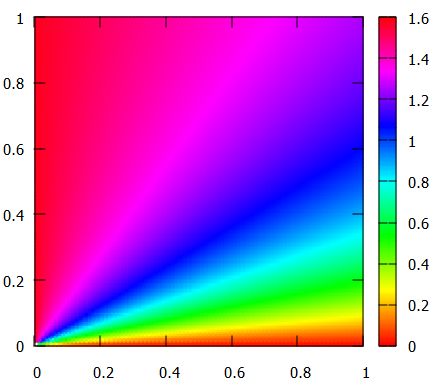
\includegraphics[width = \linewidth]{../3func/orig.png}
					\caption[.] {Интерполируемая функция}
				\end{minipage}\hfill
				\begin{minipage}{0.5\textwidth}
					\centering
					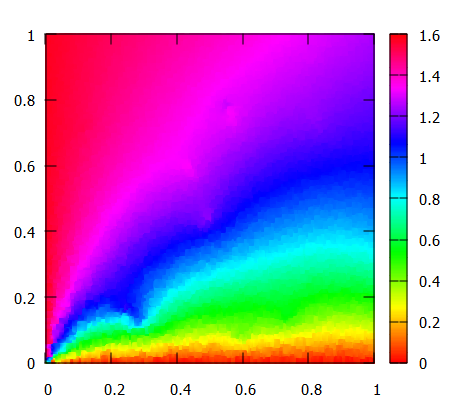
\includegraphics[width = \linewidth]{../3func/M=10T=5774Err=0.0901691.png}
					\caption[.] {Интерполяци при 10 точках}
				\end{minipage}\hfill
			\end{figure}
			\begin{figure}[H]
				\begin{minipage}{0.5\textwidth}
					\centering
					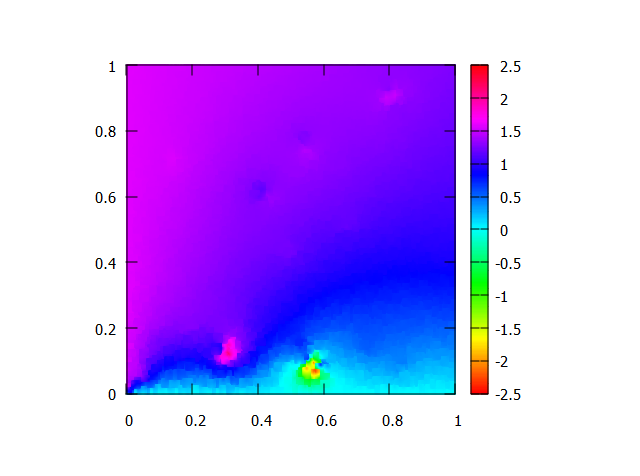
\includegraphics[width = \linewidth]{../3func/M=25T=3714Err=0.123237.png}
					\caption[.] {Интерполяция при 25 точках с редкой сеткой}
				\end{minipage}\hfill
				\begin{minipage}{0.5\textwidth}
					\centering
					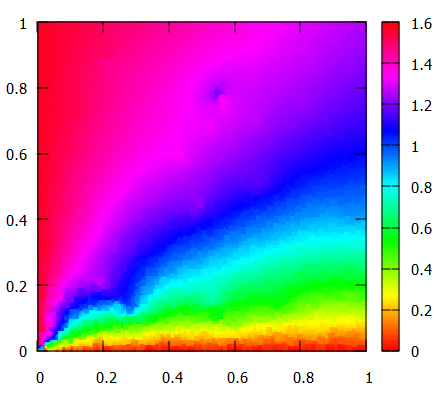
\includegraphics[width = \linewidth]{../3func/M=25T=5774Err=0.0666124.png}
					\caption[.] {Интерполяция при 25 точках}
				\end{minipage}\hfill
			\end{figure}
			\begin{figure}[H]
				\begin{minipage}{0.5\textwidth}
					\centering
					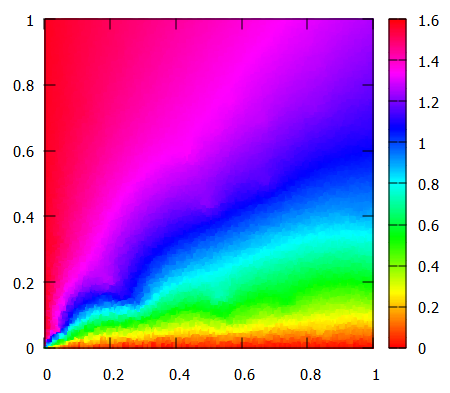
\includegraphics[width = \linewidth]{../3func/M=25T=10182Err=0.0632562.png}
					\caption[.] {Интерполяция при 25 точках с частой сеткой}
				\end{minipage}\hfill
				\begin{minipage}{0.5\textwidth}
					\centering
					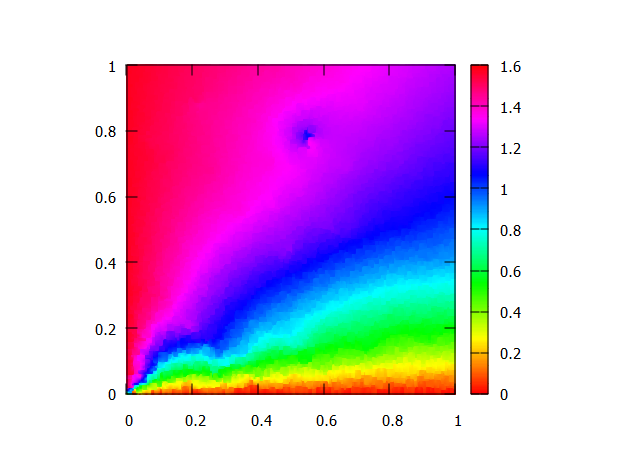
\includegraphics[width = \linewidth]{../3func/M=50T=5774Err=0.0529867.png}
					\caption[.] {Интерполяция при 50 точках}
				\end{minipage}\hfill
			\end{figure}
		
			\item \( f(x, y) = e^{10x} \)
			
			\(N = 5774\)
			\begin{table}[H]
				\centering
				\begin{tabular}{|P{5cm}|P{2.5cm}|P{2.5cm}|P{2.5cm}|P{2.5cm}|}
					\hline
					M & 10 & 25 & 50 & 100 \\ \hline
					Относительная погрешность & $0.640972$ & $0.475457$ & $0.273087$ & 0.154733\\ \hline
				\end{tabular}
			\end{table}
			
			\(M = 100\)
			\begin{table}[H]
				\centering
				\begin{tabular}{|P{5cm}|P{2.5cm}|P{2.5cm}|P{2.5cm}|}
					\hline
					N & 3718 & 5774 & 17101 \\ \hline
					Относительная погрешность & 0.458518 & 0.154733 & 0.150765\\ \hline
				\end{tabular}
			\end{table}
			
			\begin{figure}[H]
				\begin{minipage}{0.5\textwidth}
					\centering
					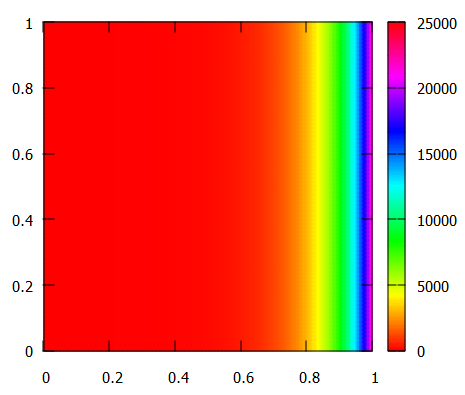
\includegraphics[width = \linewidth]{../4func/orig.png}
					\caption[.] {Интерполируемая функция}
				\end{minipage}\hfill
				\begin{minipage}{0.5\textwidth}
					\centering
					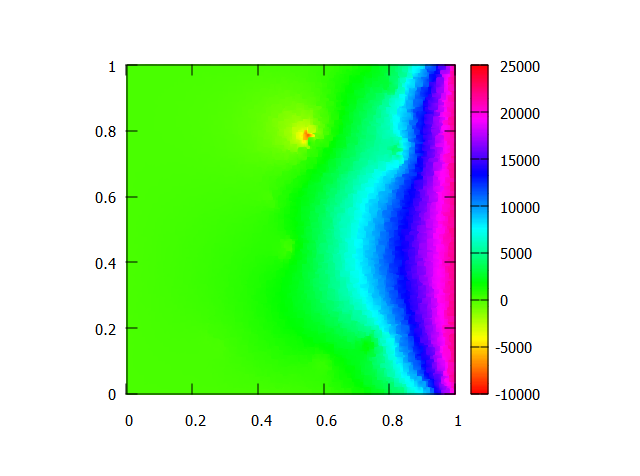
\includegraphics[width = \linewidth]{../4func/M=10T=5774Err=0.640972.png}
					\caption[.] {Интерполяци при 10 точках}
				\end{minipage}\hfill
			\end{figure}
			\begin{figure}[H]
				\begin{minipage}{0.5\textwidth}
					\centering
					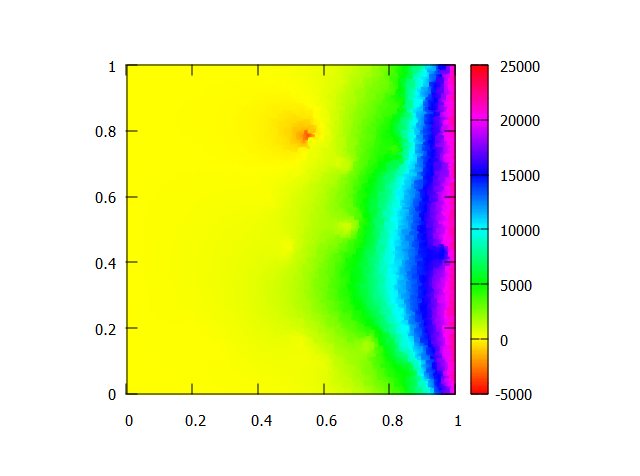
\includegraphics[width = \linewidth]{../4func/M=25T=5774Err=0.475457.png}
					\caption[.] {Интерполяция при 25 точках}
				\end{minipage}\hfill
				\begin{minipage}{0.5\textwidth}
					\centering
					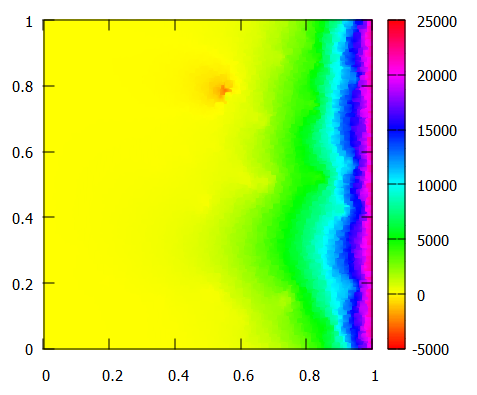
\includegraphics[width = \linewidth]{../4func/M=50T=5774Err=0.273087.png}
					\caption[.] {Интерполяция при 50 точках}
				\end{minipage}\hfill
			\end{figure}
			\begin{figure}[H]
				\begin{minipage}{0.5\textwidth}
					\centering
					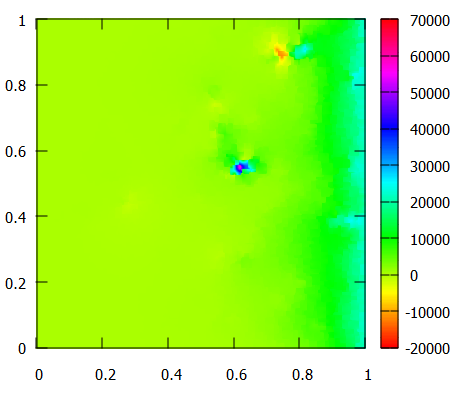
\includegraphics[width = \linewidth]{../4func/M=100T=3718Err=0.458518.png}
					\caption[.] {Интерполяция при 100 точках с редкой сеткой}
				\end{minipage}\hfill
				\begin{minipage}{0.5\textwidth}
					\centering
					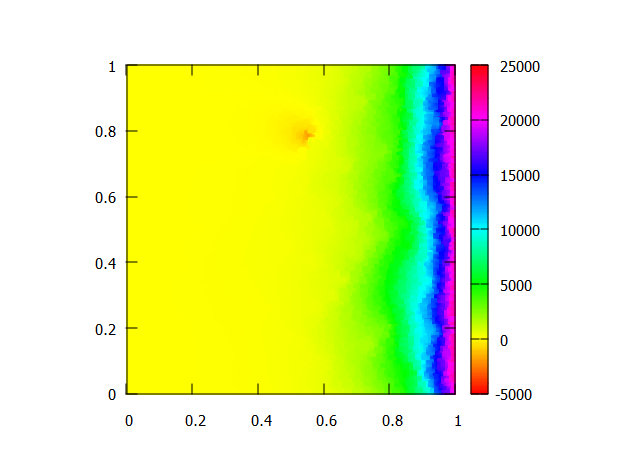
\includegraphics[width = \linewidth]{../4func/M=100T=5774Err=0.154733.png}
					\caption[.] {Интерполяция при 100 точках}
				\end{minipage}\hfill
			\end{figure}
			\begin{figure}[H]
				\centering
				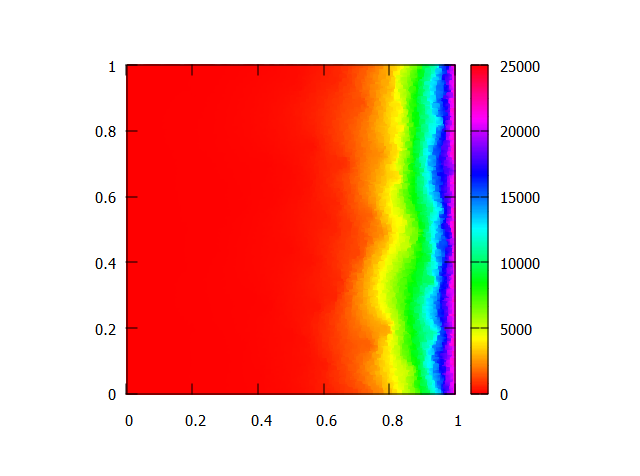
\includegraphics[width = \linewidth]{../4func/M=100T=10182Err=0.150765.png}
				\caption[.] {Интерполяция при 100 точках с частой сеткой}
			\end{figure}
		\end{enumerate}
	\section{Вывод}
		Качество интерполяции зависит от количества заданных точек и частоты сетки. На редкой сетке и при недостаточном количестве точек появляются <<всплески>>. Метод плохо интерполирует функции с большими складками, для удовлетворительного результата необходимо большое количество точек в этой области.
	\section{Литература}
	\section{Приложение}
	\lstinputlisting[language=FreeFem, caption={Код программы во FreeFem++}, captionpos=b]{../square2.edp}
	
	
\end{document}} 
